The Smartbin hardware platform is a simple construction consisting of two sensors, a microprocessor and a wifi communication module. It is embedded into a trash bin with a lid which is used
as a base for both the distance sensor and the gas sensor.

We built the prototype using an Arduino Uno board (figure \ref{fig:board}).

 As for the sensors we used a Figaro TGS2602 as our gas sensor and a MaxSonar MB1013 ultrasonic rangefinder as our distance sensor.\\
The gas sensor is a generic air quality sensor that detects variations of most of the gases listed above as "of interest" in regards to bad smell emissions.
It also detects other substances, like \ce{CO_2}  that, although odorless, are still an indicator of decomposition.\\
Even though in the course of this project we have not been able to recognise specific gases from  concentrations registered by the sensor, we make the assumption that the presence of any of the gases targeted by the sensor are valid indicators of decomposition and hence bad smell.

We use a WiFi shield on the Arduino board for wireless communication.

The presentation layer works on Android 4.0 or later.

\begin{figure}
\centering
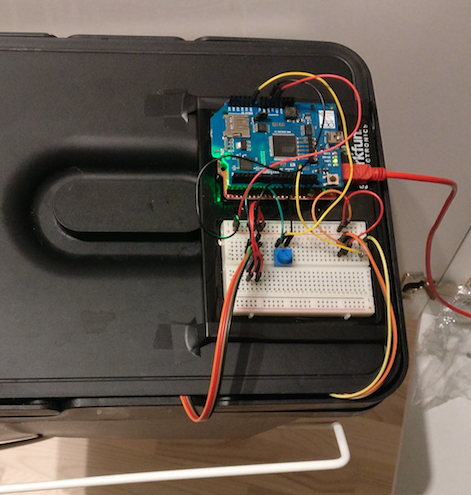
\includegraphics[scale=.3]{img/arduinoboard}
\caption{The controller board with communication shield}
\label{fig:board}
\end{figure}